\subsection{草图第二阶段}
\subsubsection{传动件的结构设计}
\begin{itemize}
	\item [a)]齿轮b结构设计
	\par 齿轮b齿顶圆直径$d_{ab}=142.5$,为了减少质量和节约材料,采用腹板式结构。考虑本设计生产批量较大,采用模锻毛坯结构,如下图所示。
	\begin{figure}[H]
		\begin{center}
			\caption{模锻毛坯齿轮}
			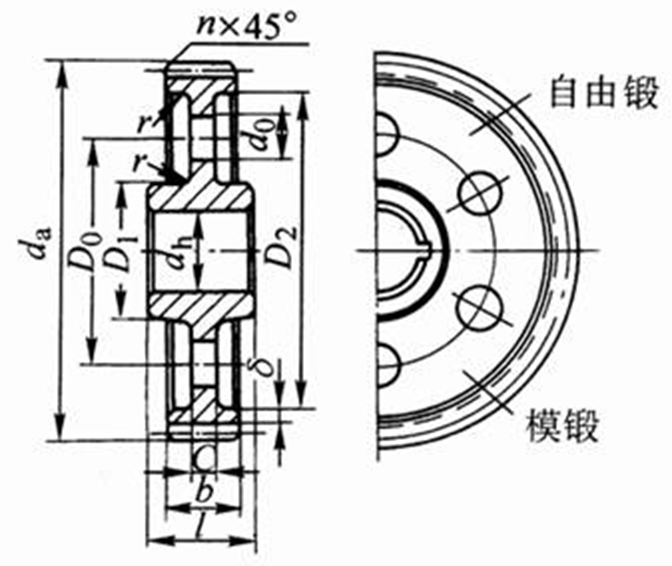
\includegraphics{pic/chilun.png}
		\end{center}
	\end{figure}
	\par 图中各尺寸如下:
		$$d_h=34$$
		$$D_1\approx 1.6d_h=54.4$$
	\par 取 $D_1=54$
		$$D_2=d_a-10=117.5$$
	\par 因为至少离齿根圆10mm,所以取$D_2=120$。
		$$c_2=\left(0.2\sim 0.3\right)b=7.6\sim 11.4$$
	\par 取$c=10$
		$$r=0.5c=5$$
		$$D_0=0.5\left(D_1+D_2\right)=87.2$$
		$$d_0\approx 0.25\left(D_2-D_1\right)=16.4$$
		$$L=\left(1.2\sim 1.5\right)d_h=40.8\approx 51$$


	\item[b)]齿轮c结构设计
	\par 齿轮3齿顶圆直径太小故做成实心式结构。
	\item[c)]齿轮d结构设计
	\par 齿轮d齿顶圆直径$d_{a2}=202$,为了减少质量和节约材料,采用腹板式结构。考虑本设计生产批量较大,采用模锻毛坯结构,如前图所示。
	\par 图中各尺寸如下:
	$$d_h=48$$
	$$D_1\approx 1.6d_h=76.8$$
	\par 取 $D_1=77$
	$$D_2=d_a-10=203.95$$
	\par 因为至少离齿根圆10mm,所以取$D_2=200$。
	$$c_2=\left(0.2\sim 0.3\right)b=12\sim 18$$
	\par 取$c=16$
	$$r=0.5c=8$$
	$$D_0=0.5\left(D_1+D_2\right)=138.5$$
	$$d_0\approx 0.25\left(D_2-D_1\right)=30.75$$
	$$L=\left(1.2\sim 1.5\right)d_h=57.6\approx 72$$
	
	
\end{itemize}
\subsubsection{轴承端盖设计}
\begin{itemize}
	\item [a)]\uppercase\expandafter{\romannumeral1}轴轴承端盖设计
	\par 由前面设计可知,轴承外径$D=52$,$d_3=8$
	$$D_2=D+\left(5\sim 5.5\right)d_3=92\sim 96$$,取$D_2=94$。
	由参考文献\cite{3}图19可知,$b=8$,取$s_3=6$。
	
	\item [b)]\uppercase\expandafter{\romannumeral2}轴轴承端盖设计
	\par 由前面设计可知,轴承外径$D=52$,$d_3=8$
	$$D_2=D+\left(5\sim 5.5\right)d_3=92\sim 96$$,取$D_2=94$。
	由参考文献\cite{3}图19可知,$b=8$,取$s_3=6$。 
	
	\item [c)]\uppercase\expandafter{\romannumeral3}轴轴承端盖设计
	\par 由前面设计可知,轴承外径$D=62$,$d_3=8$
	$$D_2=D+\left(5\sim 5.5\right)d_3=98\sim 102$$,取$D_2=100$。
	由参考文献\cite{3}图19可知,$b=8$,取$s_3=6$。
\end{itemize}
\subsubsection{套筒设计}
\begin{itemize}
	\item [a)]\uppercase\expandafter{\romannumeral1}轴套筒设计
	\par 内径$d_1=30$,外径$d_2=38$,长度$l=20$。	
	   
	\item [b)]\uppercase\expandafter{\romannumeral2}轴套筒设计
	\par 内径$d_1=30$,外径$d_2=38$,长度$l=20$。。 
	
	\item [c)]\uppercase\expandafter{\romannumeral3}轴套筒设计
	\par 内径$d_1=40$,外径$d_2=50$,长度$l=20$。
\end{itemize}

